\documentclass[tikz,border=5mm]{standalone}
\usepackage[utf8]{vietnam}
\usepackage{tikz}
\usetikzlibrary{calc,decorations.text,intersections,shapes.geometric}
%==============
\begin{document}
	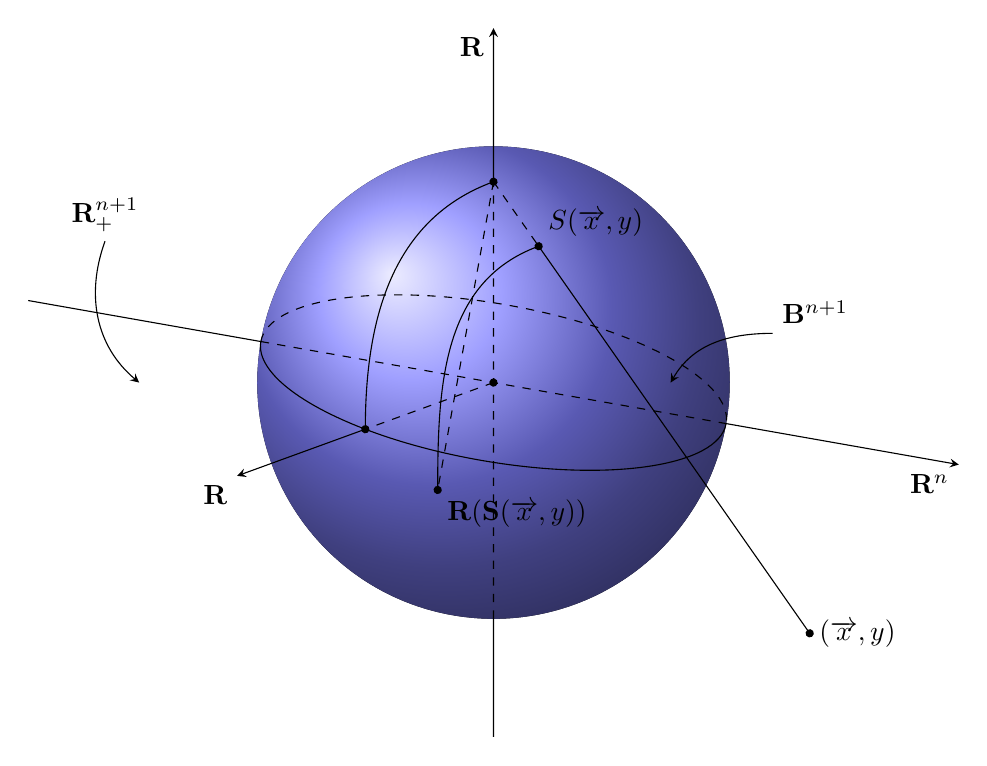
\begin{tikzpicture}
		\def\a{3}
		\def\g{10}
		\pgfmathsetmacro{\b}{\a/3}
		\begin{scope}[rotate=-\g]
			\fill[ball color=blue!50] (0:0) circle (\a);
			\draw[dashed] (180:\a) arc (180:0:{\a} and {\b}) (180:\a)--(0:\a) (-90+\g:\a)--(90+\g:0.85*\a)coordinate(Y);
			\path (Y)--++(-45:\b)coordinate(B) --++(-45:2*\a)coordinate(C) (-180:\a) arc (-180:-120:{\a} and {\b})coordinate(X);
			\draw (180:2*\a)--(180:\a)coordinate(A) (-90+\g:1.5*\a)--(-90+\g:\a) (A) arc (180:360:{\a} and {\b});
			\draw [-stealth] (Y)--(90+\g:1.5*\a)node[below left]{$\mathbf{R}$};
			\draw[-stealth](0:\a)--(0:2*\a)node[below left]{$\mathbf{R}^{n}$};
			\draw[-stealth] (X)--($2*(X)$)node[below left]{$\mathbf{R}$};
			\draw (B)node[above right]{$S(\overrightarrow{x},y)$}--(C)node[right]{$(\overrightarrow{x},y)$};
			\draw[dashed] (Y)--(B) (0:0)coordinate(O)--(X);
			\draw (Y) to[out=-150,in=90+\g] (X);
			\draw (B) to[out=-150,in=90+\g] ([shift={(-30:1.2*\b)}]X)coordinate(D)node[below right]{$\mathbf{R(S(\overrightarrow{x}},y))$};
			\draw[dashed] (Y)--(D);
			\foreach \x in {X,Y,B,C,D,O}{\fill[black] (\x) circle (1.5pt);}
			\draw[-stealth] (170:1.75*\a) node[above]{$\mathbf{R}^{n+1}_{+}$} to[out=-100,in =150] (190:1.5*\a);
			\draw[-stealth] (20:1.2*\a) node[above right]{$\mathbf{B}^{n+1}$} to [out=-170,in=70] (10 : 0.75*\a);
		\end{scope}
	\end{tikzpicture}
\end{document}